%%=====================================================================================
%%
%%       Filename:  bear.tex
%%
%%    Description:  Bear, Polar bear
%%
%%        Version:  1.0
%%        Created:  09/08/2016
%%       Revision:  none
%%
%%         Author:  Dilawar Singh (), dilawars@ncbs.res.in
%%   Organization:  NCBS Bangalore
%%      Copyright:  Copyright (c) 2016, Dilawar Singh
%%
%%          Notes:  
%%                
%%=====================================================================================

\documentclass[crop]{standalone}
%\usepackage[a4paper,landscape]{geometry}
\usepackage{tikz}
\usepackage{pgfplots}
\usepgfplotslibrary{polar}
\usetikzlibrary{positioning}
\begin{document}

\begin{tabular}{c c}
    Bear & Polar Bear \\
\begin{tikzpicture}[ ]
\begin{axis}[
        grid = both
        , minor tick num=5
        , grid style={draw=gray!10,line width=.1pt}
        , major grid style={line width=0.5pt,draw=gray!50}
        , axis line style={latex-latex}
        , xticklabels = \empty
        , yticklabels = \empty
        , draw=blue!20
    ]

        \addplot[draw=none] coordinates {(2,2)};
        \node[] (image) at (rel axis cs:0.5,0.5) {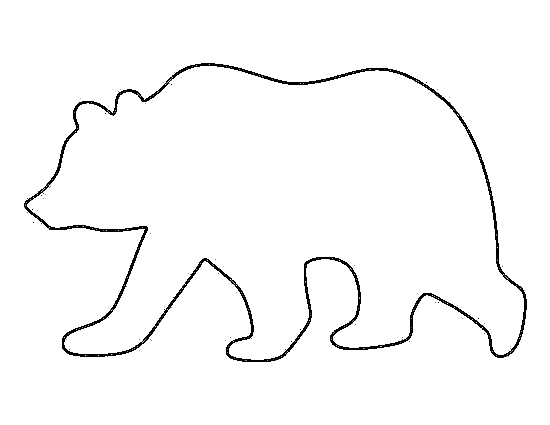
\includegraphics[width=5cm]{./bear.png}};
    \end{axis}
\end{tikzpicture} &
\begin{tikzpicture}[]
    ]
    \begin{polaraxis}[
        grid = both
        , minor tick num=5
        , grid style={draw=gray!10,line width=.1pt}
        , major grid style={line width=0.5pt,draw=gray!50}
        , axis line style={latex-latex}
        , xticklabels = \empty
        , yticklabels = \empty
        , draw=blue!20
    ]
        \addplot[draw=none] coordinates {(1,1)};
        \node[] at (rel axis cs:0,0) {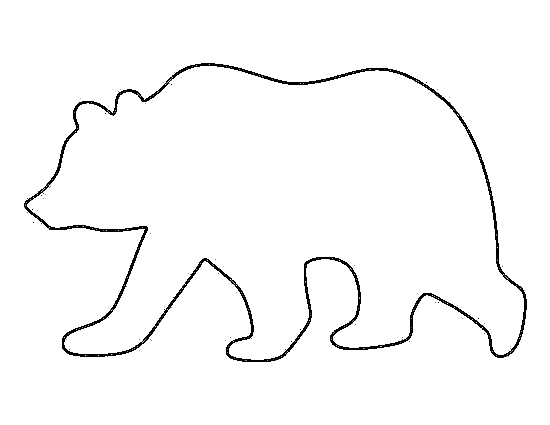
\includegraphics[width=5cm]{./bear.png}};
    \end{polaraxis}
\end{tikzpicture}%
\end{tabular}

\end{document}

